% !TEX root = ../main.tex

\section{Data and Model}

\begin{frame}[shrink=12]{Data Sources, License, and Split}
  \begin{columns}[T]
    \column{0.52\textwidth}
    \begin{block}{Sources}
      \small
      \begin{itemize}
        \item TempQuestions: English temporal QA benchmark, 1,271 questions~\parencite{jia2018tempquestions}
        \item Freebase: archived KB, CC-BY data dump~\parencite{bollacker2008freebase}
        \item idirlab/freebases: CC0-1.0 processed mirror used for v1 facts
        \item FACC1/ELQ-style assets: entity retrieval support, not redistributed
      \end{itemize}
    \end{block}
    \column{0.44\textwidth}
    \begin{exampleblock}{Locked split policy}
      \small
      \begin{itemize}
        \item canonical TempQuestions: 888 train / 383 test
        \item v1 synthetic training pool: 2,061 examples
        \item tuning split: 1,855 train / 206 validation
        \item final evaluation artifact: 268 human test questions
      \end{itemize}
    \end{exampleblock}
  \end{columns}
  \vspace{0.1cm}
  \begin{alertblock}{Data reality}
    The bundled human TempQuestions path is partially corrupted, so v1 training uses filtered synthetic temporal supervision and keeps the human test artifact held out.
  \end{alertblock}
\end{frame}

\begin{frame}[shrink=6]{Data Pipeline and Cleaning}
  \begin{columns}[T]
    \column{0.55\textwidth}
    \begin{block}{Pipeline}
      \small
      \begin{enumerate}
        \item audit TempQuestions and merged artifacts
        \item mine / normalize temporal facts
        \item generate synthetic temporal samples
        \item filter by quality and operator distribution
        \item export ChatKBQA instruction-tuning format
      \end{enumerate}
    \end{block}
    \column{0.41\textwidth}
    \begin{exampleblock}{Cleaning targets}
      \small
      \begin{itemize}
        \item placeholder-collapsed SPARQL
        \item suspicious merged records
        \item missing date literals
        \item noisy relation patterns
      \end{itemize}
    \end{exampleblock}
  \end{columns}
  \vspace{0.15cm}
  \begin{alertblock}{Design principle}
    Treat data quality as a first-class engineering artifact, not as hidden preprocessing.
  \end{alertblock}
\end{frame}

\begin{frame}[shrink=10]{T-ChatKBQA vs.\ ChatKBQA Baseline}
  \begin{center}
    \vspace{-0.2cm}
    \definecolor{indigo}{RGB}{63, 81, 181}
\definecolor{emerald}{RGB}{0, 135, 90}

\begin{tikzpicture}[
    node distance=0.08cm,
    boxblue/.style={
        draw=indigo!60!black, fill=indigo!4!white, rounded corners=3pt,
        text width=1.4cm, minimum height=0.55cm, align=center, font=\fontsize{5.5}{6.5}\selectfont\sffamily, inner sep=3pt, thick
    },
    boxteal/.style={
        draw=teal!70!black, fill=teal!4!white, rounded corners=3pt,
        text width=1.4cm, minimum height=0.55cm, align=center, font=\fontsize{5.5}{6.5}\selectfont\sffamily, inner sep=3pt, thick
    },
    boxorange/.style={
        draw=orange!80!black, fill=orange!5!white, rounded corners=3pt,
        text width=1.4cm, minimum height=0.55cm, align=center, font=\fontsize{5.5}{6.5}\selectfont\sffamily, inner sep=3pt, thick
    },
    arrowblue/.style={-Stealth, indigo!60!black, thick},
    arrowteal/.style={-Stealth, teal!60!black, thick},
    groupblue/.style={draw=indigo!25, fill=indigo!1!white, dashed, rounded corners=6pt, inner sep=6pt},
    groupteal/.style={draw=teal!30, fill=teal!1!white, dashed, rounded corners=6pt, inner sep=6pt},
    badgeblue/.style={draw=indigo!40!black, fill=indigo!10, rounded corners=2pt, inner sep=1.5pt, font=\fontsize{4.5}{5.5}\selectfont\bfseries\sffamily, text=indigo!80!black},
    badgeteal/.style={draw=teal!40!black, fill=teal!10, rounded corners=2pt, inner sep=1.5pt, font=\fontsize{4.5}{5.5}\selectfont\bfseries\sffamily, text=teal!80!black},
]

% ============================================================
% BASELINE ChatKBQA (top) -- with gap for alignment
% ============================================================
\begin{scope}[local bounding box=baseline]
    \node[boxblue] (B0) {NL\\Question};
    \node[boxblue, right=1.7cm of B0] (B1) {LLaMA-2\\+ LoRA SFT\\(static)};
    \node[boxblue, right=0.15cm of B1] (B2) {Entity/Rel\\Retrieval\\FACC1+ELQ};
    \node[boxblue, right=0.15cm of B2] (B3) {SPARQL\\Exec\\Freebase};
    \node[boxblue, right=0.15cm of B3] (B4) {Answer};

    \draw[arrowblue] (B0) -- (B1);
    \draw[arrowblue] (B1) -- (B2);
    \draw[arrowblue] (B2) -- (B3);
    \draw[arrowblue] (B3) -- (B4);
\end{scope}

\begin{pgfonlayer}{background}
    \node[groupblue, fit=(B0)(B1)(B2)(B3)(B4),
          label={[indigo!70!black, font=\tiny\bfseries\sffamily]above:CHATKBQA BASELINE (ACL 2024)}] (G1) {};
\end{pgfonlayer}

% ============================================================
% T-ChatKBQA (bottom) -- perfectly aligned below baseline
% ============================================================
\begin{scope}[local bounding box=temporal]
    \node[boxorange, below=1.6cm of B0] (T0) {NL Temporal\\Question};
    \node[boxteal, right=0.15cm of T0] (T1) {Agent\\Router\\(before/after)};
    \node[boxteal, right=0.15cm of T1] (T2) {LLaMA-2+LoRA\\SFT (temp.)\\{\fontsize{4.5}{5.5}\selectfont TC,ARGMAX/MIN}};
    \node[boxteal, right=0.15cm of T2] (T3) {Extended\\Retrieval\\Ent+Rel+TS};
    \node[boxteal, right=0.15cm of T3] (T4) {Temporal\\SPARQL\\Freebase};
    \node[boxorange, right=0.15cm of T4] (T5) {Answer +\\Provenance};

    \draw[arrowteal] (T0) -- (T1);
    \draw[arrowteal] (T1) -- (T2);
    \draw[arrowteal] (T2) -- (T3);
    \draw[arrowteal] (T3) -- (T4);
    \draw[arrowteal] (T4) -- (T5);

    % Δ pill badge annotations snuggly positioned above the boxes
    \node[badgeblue] (D1) at ($(T1.north)+(0,0.28)$) {$\Delta_1$: Router};
    \node[badgeteal] (D2) at ($(T2.north)+(0,0.28)$) {$\Delta_2$: Operators};
    \node[badgeteal] (D3) at ($(T3.north)+(0,0.28)$) {$\Delta_3$: Timestamp};
    \node[badgeteal] (D4) at ($(T4.north)+(0,0.28)$) {$\Delta_4$: Temp. SPARQL};

    % Premium structured database input block for training data
    \node[draw=teal!70!black, fill=teal!5, rounded corners=2.2pt,
          text width=1.8cm, minimum height=0.35cm, align=center,
          font=\fontsize{4.5}{5.5}\selectfont\bfseries\sffamily, text=teal!80!black] (Db) at ($(T2.south)-(0,0.55cm)$) {Synth. Temporal Data\\(2,061 examples)};
    \draw[-Stealth, teal!70!black, thick] (Db) -- (T2);
\end{scope}

\begin{pgfonlayer}{background}
    \node[groupteal, fit=(T0)(T1)(T2)(T3)(T4)(T5)(D1)(D2)(D3)(D4),
          label={[teal!70!black, font=\tiny\bfseries\sffamily]above:T-CHATKBQA (THIS WORK) --- GENERATE-THEN-RETRIEVE + TEMPORAL}] (G2) {};
\end{pgfonlayer}

% ============================================================
% LEGEND (below T-ChatKBQA group on the right)
% ============================================================
\node[draw=black!15, fill=black!2!white, rounded corners=4pt, inner sep=4pt,
      font=\fontsize{4.5}{5.5}\selectfont\sffamily,
      anchor=north east, yshift=-0.15cm] at (G2.south east)
    {\begin{tabular}{ll}
      $\Delta_{1-4}$ & Novel temporal contributions \\
      TC             & Temporal Constraint (during) \\
      ARGMAX/MIN     & Superlative (last/first) \\
      gt/ge/lt/le    & Comparison (before/after) \\
    \end{tabular}};

\end{tikzpicture}

  \end{center}
\end{frame}

\begin{frame}[shrink=12]{Model Selection and Tuning}
  \begin{columns}[T]
    \column{0.52\textwidth}
    \begin{block}{Chosen model}
      \small
      \begin{itemize}
        \item LLaMA-2-7B generator~\parencite{touvron2023llama}
        \item LoRA adaptation~\parencite{hu2022lora}
        \item ChatKBQA-compatible S-expression output
      \end{itemize}
    \end{block}
    \begin{block}{Final config}
      \small 5 epochs, 5e-5 learning rate, effective batch 16, beam size 5, max 256 new tokens.
    \end{block}
    \column{0.44\textwidth}
    \begin{exampleblock}{Basic tuning}
      \small
      Compared 3/5/10 epochs, 3e-5/5e-5/1e-4 learning rates, and beam 3/5/8 using the synthetic validation split. The selected run balanced syntax validity, stability, and runtime.
    \end{exampleblock}
  \end{columns}
  \vspace{0.1cm}
  \begin{alertblock}{Verified run artifact}
    Training completed for 645 steps on 2,061 synthetic examples; reported values follow run artifacts, not stale template defaults.
  \end{alertblock}
\end{frame}

\section{Evaluation}

\begin{frame}[shrink=7]{Evaluation Setup and Baselines}
  \begin{center}
    \scriptsize
    \setlength{\tabcolsep}{4pt}
    \resizebox{\textwidth}{!}{%
    \begin{tabular}{lccp{4.7cm}}
      \toprule
      \textbf{Method} & \textbf{Same Dataset?} & \textbf{Role} & \textbf{Why included} \\
      \midrule
      Generate-only & Yes & Main baseline & Measures raw temporal generator without effective grounding \\
      + fuzzy relation grounding & Yes & Ablation & Tests whether retrieval can repair hallucinated relations \\
      + golden entity & Yes & Oracle ablation & Separates entity grounding from relation and KB coverage failures \\
	      ChatKBQA paper~\parencite{luo2024chatkbqa} & No & Reference only & Source-framework scale: WebQSP 79.8 F1 / 83.2 Hits@1 / 73.8 Acc \\
      \bottomrule
    \end{tabular}
    }
  \end{center}
  \vspace{0.15cm}
  \begin{alertblock}{Baseline statement}
    The main baseline is the same-dataset generate-only pipeline on TempQuestions~\parencite{jia2018tempquestions}; ChatKBQA paper numbers are reference-only because they use different datasets.
  \end{alertblock}
\end{frame}

\begin{frame}[shrink=5]{Diagnostic Results}
  \begin{center}
    \scriptsize
    \setlength{\tabcolsep}{5pt}
    \resizebox{\textwidth}{!}{%
    \begin{tabular}{lcp{6.2cm}}
      \toprule
      \textbf{Stage} & \textbf{Value} & \textbf{Interpretation} \\
      \midrule
      Generation validity & 87.6\% & the model often emits structurally usable S-expressions \\
      Grounded relation+entity pairs & 5 / 995 & most parser-valid predictions cannot be grounded in the KB \\
      Questions with KB answers & 1 / 268 & execution rarely returns an answer \\
      F1 / Hits@1 / Accuracy & 0.0 / 0.0 / 0.0 & answer-level quality is blocked by grounding and coverage \\
      \bottomrule
    \end{tabular}
    }
  \end{center}
  \vspace{0.15cm}
  \begin{alertblock}{Key interpretation}
    The pipeline does not fail first at syntax generation. It fails at relation grounding, entity grounding, and KB execution coverage.
  \end{alertblock}
\end{frame}

\begin{frame}[shrink=8]{What Works vs.\ What Fails}
  \begin{columns}[T]
    \column{0.48\textwidth}
    \begin{block}{Works}
      \small
      \begin{itemize}
        \item end-to-end training and inference complete
        \item high valid S-expression diagnostic rate
        \item API/CLI/Streamlit/Docker surfaces exist
        \item evaluation isolates failure stages
      \end{itemize}
    \end{block}
    \column{0.48\textwidth}
    \begin{alertblock}{Fails}
      \small
      \begin{itemize}
        \item generated relations hallucinate beyond the KB
        \item entity IDs often point to the wrong entity
        \item narrow 22-relation training slice limits coverage
        \item raw answer-level score remains 0.0
      \end{itemize}
    \end{alertblock}
  \end{columns}
  \vspace{0.15cm}
  \begin{exampleblock}{Ablation takeaway}
    Fuzzy relation grounding raises relation match sharply, golden entities improve answer rate, but F1 remains zero; v2 needs retrieval-constrained generation plus broader relation/fact coverage.
  \end{exampleblock}
\end{frame}

\section{Deployment and Operations}

\begin{frame}{Deployment Surfaces and Live Requirements}
  \begin{columns}[T]
    \column{0.48\textwidth}
    \begin{block}{Primary surfaces}
      \small
      \begin{itemize}
        \item FastAPI for programmatic inference
        \item CLI for reproducible local checks
        \item Docker for packaging
        \item Streamlit for presentation and inspection
      \end{itemize}
    \end{block}
    \column{0.48\textwidth}
    \begin{exampleblock}{Full live requirements}
      \small
      \begin{itemize}
        \item base LLaMA model
        \item LoRA adapter checkpoint
        \item Freebase/Virtuoso backend
        \item entity/relation retrieval assets
      \end{itemize}
    \end{exampleblock}
    \begin{alertblock}{Demo policy}
      \small Missing assets trigger explicit degraded/offline mode instead of a fake live answer.
    \end{alertblock}
  \end{columns}
\end{frame}

\begin{frame}{Streamlit Demo Screenshot}
  \begin{center}
    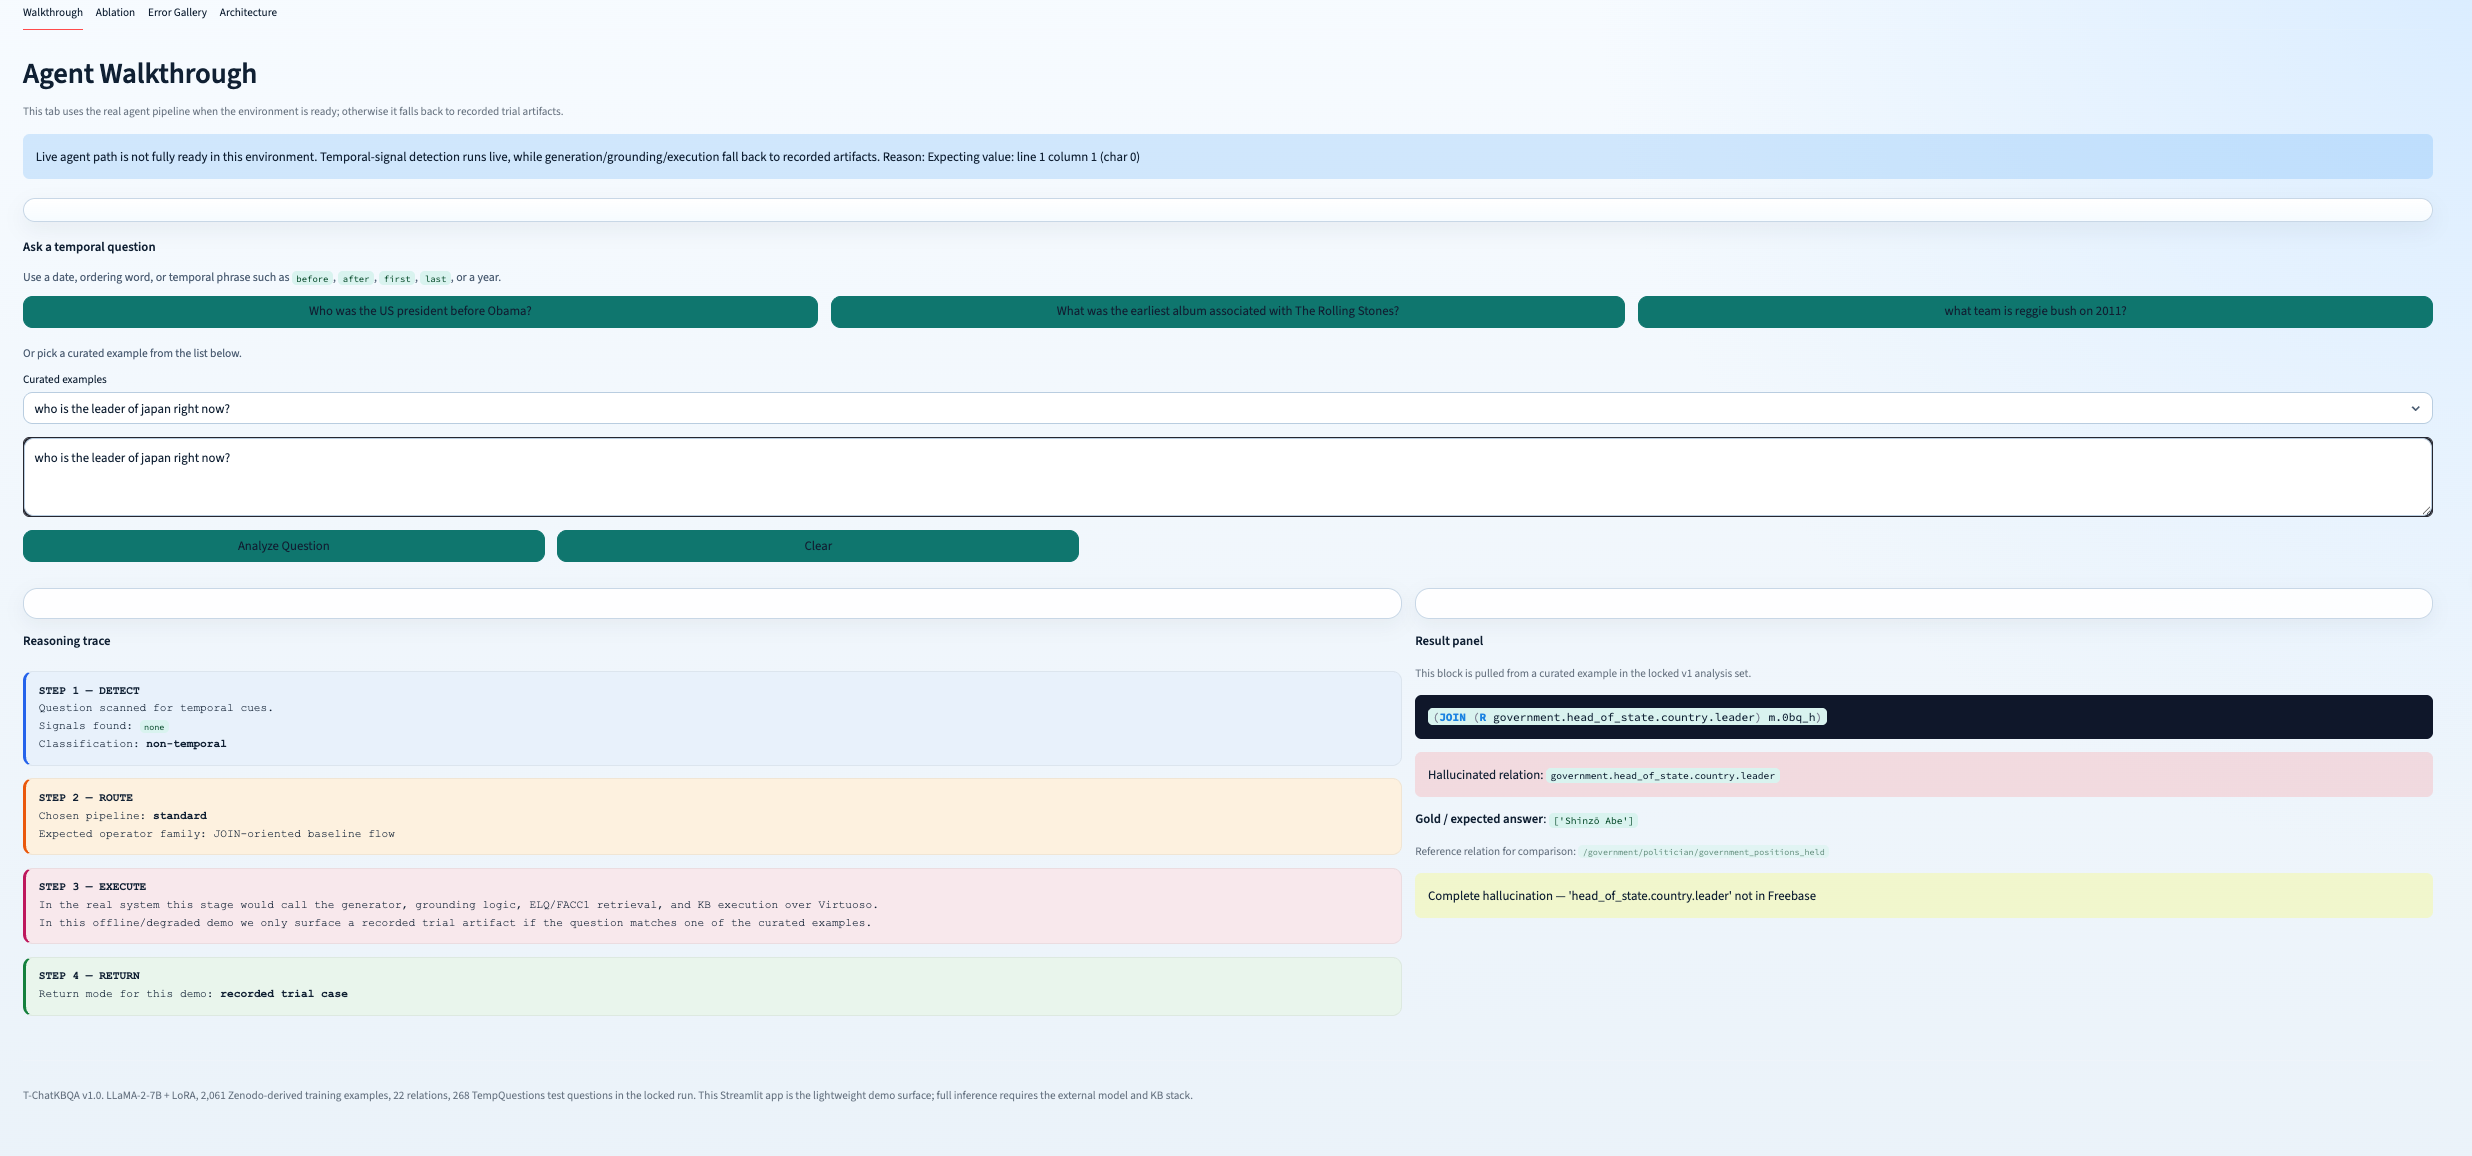
\includegraphics[width=\textwidth]{../images/streamlit_example.png}
  \end{center}
\end{frame}

\begin{frame}[shrink=8]{Agentic Workflow}
  \begin{columns}[T]
    \column{0.48\textwidth}
    \begin{block}{Agent steps}
      \small
      \begin{enumerate}
        \item detect temporal signals
        \item route to temporal or standard path
        \item execute first attempt
        \item retry with relaxed constraints if empty
        \item return answer plus provenance
      \end{enumerate}
    \end{block}
    \begin{alertblock}{Why this is useful}
      The system exposes intermediate decisions instead of returning an opaque answer string.
    \end{alertblock}
    \column{0.48\textwidth}
    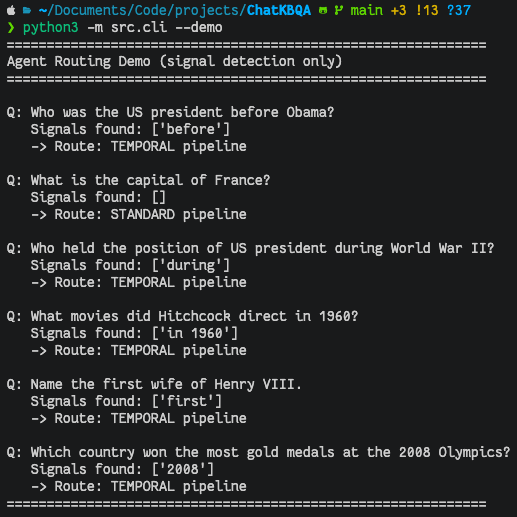
\includegraphics[width=0.72\linewidth]{../images/CLI_demo.png}
    \vspace{0.08cm}
    \begin{exampleblock}{Visible provenance}
      \small
      \begin{itemize}
        \item temporal signals
        \item generated logical form
        \item SPARQL when available
        \item retry count and reasoning trace
      \end{itemize}
    \end{exampleblock}
  \end{columns}
\end{frame}

\begin{frame}[shrink=8]{Monitoring, Privacy, and Robustness}
  \begin{columns}[T]
    \column{0.32\textwidth}
    \begin{block}{Monitoring}
      \small
      \begin{itemize}
        \item answer rate
        \item retry rate
        \item latency percentiles
        \item executor errors
      \end{itemize}
    \end{block}
    \column{0.32\textwidth}
    \begin{block}{Privacy}
      \small
      \begin{itemize}
        \item public benchmark data
        \item minimize query logs
        \item avoid PII retention
      \end{itemize}
    \end{block}
    \column{0.32\textwidth}
    \begin{block}{Robustness}
      \small
      \begin{itemize}
        \item OOD questions
        \item non-English inputs
        \item vague time wording
        \item missing KB facts
      \end{itemize}
    \end{block}
  \end{columns}
  \vspace{0.15cm}
  \begin{alertblock}{Responsible-use note}
    The system is more auditable than a free-form chatbot, but it inherits KB staleness, dataset bias, and model uncertainty.
  \end{alertblock}
\end{frame}

\section{Closeout}

\begin{frame}[shrink=8]{Key Takeaways and Future Work}
  \begin{columns}[T]
    \column{0.5\textwidth}
    \begin{block}{Submission-ready}
      \small
      \begin{itemize}
        \item temporal KBQA architecture implemented
        \item data pipeline and tooling documented
        \item training/inference/evaluation completed
        \item deployable API/CLI/Streamlit surfaces
      \end{itemize}
    \end{block}
    \column{0.46\textwidth}
    \begin{exampleblock}{Next engineering priorities}
      \small
      \begin{itemize}
        \item retrieval-constrained generation
        \item stronger entity linker integration
        \item broader relation/fact coverage
        \item benchmark regression gate before promotion
      \end{itemize}
    \end{exampleblock}
  \end{columns}
  \vspace{0.15cm}
  \begin{alertblock}{Final message}
    The v1 system is submission-ready as an engineering artifact, but not performance-ready as a production QA model.
  \end{alertblock}
\end{frame}
